\documentclass[stu, 12pt, letterpaper, donotrepeattitle, floatsintext, natbib]{apa7}
\usepackage[utf8]{inputenc}
%\usepackage{fontspec} %paquete para usar la fuente Arial 12
%\usepackage{comment}
\usepackage{marvosym}
\usepackage{graphicx}
\usepackage{float}
\usepackage[normalem]{ulem}
\usepackage[spanish]{babel}
\usepackage{listings} 
\usepackage{lastpage} %para le formato que quiere la profe QUITAR SI QUIERES OG APA7
\usepackage{ragged2e} %para le formato que quiere la profe QUITAR SI QUIERES OG APA7
\usepackage{indentfirst} %para le formato que quiere la profe QUITAR SI QUIERES OG APA7

%comando para ajustar la fuente Arial en todo el documento
%\setmainfont{Arial} %COMPILAR DOC CON XeLateX DOS VECES

%\DeclareCaptionLabelSeparator*{spaced}{\\[2ex]}
%\captionsetup[table]{textfont=it,format=plain,justification=justified,
%  singlelinecheck=false,labelsep=spaced,skip=1pt}

% Define a custom color
\definecolor{backcolour}{rgb}{0.95,0.95,0.92}
\definecolor{codegreen}{rgb}{0,0.6,0}

% Define a custom style
\lstset{
    backgroundcolor=\color{backcolour},   
    commentstyle=\color{codegreen},
    basicstyle=\ttfamily\footnotesize,
    breakatwhitespace=false,         
    breaklines=true,                 
    keepspaces=true,                 
    numbers=left,       
    numbersep=5pt,                  
    showspaces=false,                
    showstringspaces=false,
    showtabs=false,                  
    tabsize=2,
}

\selectlanguage{spanish}

\useunder{\uline}{\ul}{}
\newcommand{\myparagraph}[1]{\paragraph{#1}\mbox{}\\}

%\rfoot{Página \thepage \hspace{1pt} de \pageref{LastPage}}%QUITAR SI QUIERES OG APA7 
\rhead{} %QUITAR SI QUIERES OG APA7
\setcounter{secnumdepth}{3} %permite enumerar las secciones QUITAR SI QUIERES OG APA7
\setlength{\parindent}{1.27cm} %sangria forzada QUITAR SI QUIERES OG APA7

\renewcommand\labelitemi{\(\bullet\)}

\newcommand*\chem[1]{\ensuremath{\mathrm{#1}}}

\begin{document}
    %PORTADA
    \begin{titlepage}
        \begin{figure}[ht]
            \centering
            
\includegraphics[width=15cm]{logosITT.png}
        \end{figure}
        \centering
        {\Large Tecnológico Nacional de México\\Instituto Tecnológico de Tijuana\par}
        \vspace{1cm}
        {\Large SCD-1015SC6C Lenguajes y Automatas I\par}
        \vspace{1cm}
        {\Large Unidad 2\par}
        \vspace{1.5cm}
        {\Large\bfseries Práctica 1\par}
        \vspace{2cm}
        {\large Lic. Gloria Leticia Morales Rios\par}
        \vfill
            {\large Abraham Jhared Flores Azcona, 19211640\par}
        \vfill
        {\large 25 de marzo de 2022}
    \end{titlepage}

% Índices
\pagenumbering{arabic}
    % Contenido
\renewcommand\contentsname{Contenido}
\tableofcontents

% Cuerpo 
    %NOTA: PARA CITAR ESTILO "Merts (2003)" usar \cite{<nombre_cita_bib>}
    %                        "(Metz, 1978)" usar \citep{<nombre_cita_bib>}
\newpage
\section{Introducción}
Como \begin{justifying}
    parte relevante de los estudios correspondientes a Lenguajes y Autómatas,
    las expresiones regulares nos permiten buscar cadenas que cumplen ciertas
    caracterísicas e inclusive modificarlas acorde a dichas reglas. Sin embargo,
    un problema severo es aquel de cómo aplicarlas. En esta breve práctica se
    siguen los pasos del video adjunto para utilizar la libreria interna del
    lenguaje Java para demostrar ciertas expresiones regulares y su funcionamiento
    en las cadenas propuestas.
    \end{justifying}
\vspace{\baselineskip}
\section{Práctica}
Como \begin{justifying}
se mencionó anteriormente, utilizaremos el lenguaje Java para las expresiones
    regulares, debido a que es una opción muy cómoda para emplear, aparte de que el video
    adjunto a la asignación muestra el código completo y explica cada una de sus partes.
\end{justifying}
En \begin{justifying}
    este caso, los cuatro archivos de código expuestos en el video fueron adjuntados
    en un solo archivo para facilitar la compresión del código, así com expresarlo 
    en un solo bloque dentro de éste documento.\par
\end{justifying}
\begin{lstlisting}[language=Java]
//libreria para el manejo de regex por medio de wildcards
import java.util.regex.*;

public class App {
    static void ejemplo1() {
        //declaracion del patron
        String patron = "a[mp]";
        Pattern p = Pattern.compile(patron);

        //texto de prueba
        String texto = "Estamos aprendiendo a usar expresiones regulares!";
        Matcher coincidencia = p.matcher(texto);

        //despliegue
        String resultado = coincidencia.replaceAll("x");
        System.out.println("EJEMPLO 1 \n\n" + resultado + "\n");
    }

    static void ejemplo2() {
        //declaracion del patron
        String patron = "[0-9]+";
        Pattern p = Pattern.compile(patron);

        //texto de prueba
        String texto = "uno1dos2tres3cuatro4";

        //despliegue
        String[] coincidencias = p.split(texto);
        System.out.println("EJEMPLO 2\n");
        for (String s : coincidencias) {
            System.out.println(s);
        }
        System.out.println();
    }

    static void ejemplo3() {
        //declaracion del patron
        String patron = "[s]";
        Pattern p = Pattern.compile(patron);

        //texto de prueba
        String texto = "Estamos aprendiendo a usar expresiones regulares!";
        Matcher coincidencia = p.matcher(texto);

        //despliegue
        System.out.println("EJEMPLO 3\n");
        while (coincidencia.find()) {
            System.out.printf(
                "Encontrado %s en la posicion %d y acaba en %d\n",
                coincidencia.group(),
                coincidencia.start(),
                coincidencia.end()
            );
        }
        System.out.println();
    }

    static void ejemplo4() {
        //declaracion del patron
        String patron = "[a-m&&h-z]";
        Pattern p = Pattern.compile(patron);

        //texto de prueba
        String texto = "h";
        Matcher coincidencia = p.matcher(texto);

        //despliegue
        System.out.println("EJEMPLO 4\n");
        if (coincidencia.matches()) {
            System.out.println("Coincide!!!\n");
        }
        else {
            System.out.println("No coincide!!!\n");
        }
    }

    public static void main(String[] args) throws Exception {
        System.out.println("Practica 1 U2 - Lenguajes y Automatas\n");
        ejemplo1();
        ejemplo2();
        ejemplo3();
        ejemplo4();
    }
}  
\end{lstlisting}
\vspace{\baselineskip}
\subsection{Ejemplo 1}
En el \begin{justifying}
     ejemplo 1, estamos usando el patrón \(a[mp]\) para destacar todas aquellas cadenas
     donde \(a\) está seguida de \(m\) ó \(p\); en seguida reemplaza dichas ocurrencias con la letra 
     \(x\) produciendo el resultado esperado.\par
 \end{justifying}
 \begin{figure}[H]
    \centering
    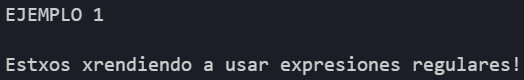
\includegraphics[\textwidth]{ejemplo1.jpg}
\end{figure}
\subsection{Ejemplo 2}
A    \begin{justifying}
    grandes rasgos, la expresión \([0-9]+\) nos hace saber que resaltemos
    aquellas coincidencias donde se comienze con cualquier valor decimal
    de un solo dígito, concatenado por cualquier cadena. Posteriormente, filtramos
    la cadena de muestra acorde a la coincidencia, que nos despliega aquellas cadenas
    que no sean un solo dígito decimal.\par
    \end{justifying}
    \begin{figure}[H]
        \centering
        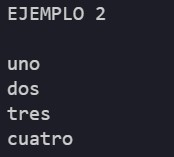
\includegraphics[height=4cm]{ejemplo2.jpg}
    \end{figure}
\subsection{Ejemplo 3}
En  \begin{justifying}
    este ejemplo, el patrón \([s]\) nos indica que queremos encontrar solamente 
    la letra \(s\) dentro del alfabeto para poder encontrarla a lo largo de la cadena
    ejemplo. En este caso, desplegaremos todas sus ocurrencias a lo largo de la cadena;
    especificamente desde donde empieza dicha coincidencia hasta donde termina.\par
    \end{justifying}
    \begin{figure}[H]
        \centering
        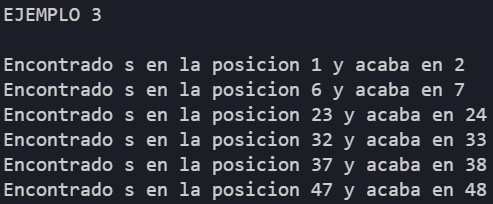
\includegraphics[height=6cm]{ejemplo3.jpg}
    \end{figure}
\vspace{\baselineskip}
\subsection{Ejemplo 4}
Finalmente, \begin{justifying}
        en el ejemplo 4, el patrón \([a-m\&\&h-z]\) nos indica que busquemos
        aquellas coincidencias donde se encuentre desde la letra \(a\) hasta la \(m\)
        y desde la \(h\) hasta la \(z\). Los \(\&\&\) indican conjunción, por lo que
        dicha expresión se puede reducir a \([a-z]\), que se puede interpretar como 
        encontrar una coincidencia de cualquier letra minúscula del alfabeto latino.\par
    \end{justifying}
    \begin{figure}[H]
        \centering
        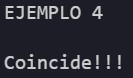
\includegraphics[height=4cm]{ejemplo4.jpg}
    \end{figure}
\section{Conclusión}
Las \begin{justifying}
    expresiones regulares (\emph{regex} por su nombre en inglés) nos permite analizar
    cadenas para poderles realizar distintas operaciones programaticas que nos permiten
    facilitarnos la vida en cuestiones digitales. El poder manejarlas de primera mano
    nos permite comprender su alcanze y darnos un mejor entendimiento para aplicarlas en nuestros
    proyectos de programación.\par   
    \end{justifying}
\end{document}